También conocido como \emph{Método de Newton-Raphson}.
Este método, es un de los más usados y efectivos que existen; en comparación a otros métodos,
el método de \emph{Newton-Raphson} no trabaja sobre un intervalo sino que basa su fórmula en un \emph{proceso iterativo}
al igual que el \emph{Método de Lipschitz o de iteración de punto fijo.}.

Para realizar una descripción del presente método,
supongamos que tenemos una aproximación $x_{i}$ a la raíz $x_{y}$,
de una función determinada $f(x)$,

\begin{center}
	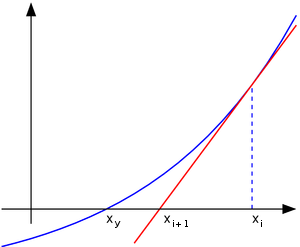
\includegraphics[width=150px]{img/newton}
\end{center}

Ahora si trazamos la recta tangente a la curva en el punto $(x_{i},f(x_{i}))$,
ésta va a cruzar el eje $x$ en un punto $x_{i+1}$,
que será nuestra siguiente aproximación a la raíz $x_{y}$.

Por otro lado, para calcular el punto $x_{i+1}$, calculamos primero la ecuación de la recta tangente.
Tenemos que la pendiente es:
$$m=f'(x_{i})$$
Por lo tanto la ecuación de la recta tangente a nuestra curva queda dada por:
$$y-f(x_{i}) = f'(x_{i})(x-x_{i})$$.

Ahora podemos asumir el valor de $y$, como $y=0$ y tenemos
$$-f(x_{i}) = f'(x_{i})(x-x_{i}),$$
despejando $x$, tenemos:
$$x=x_{i+1}=x_{i}-\frac{f(x_{i})}{f'(x_{i})},\ si\ f'(x_{i}) \neq 0$$

Como decíamos en un principio, el método de \emph{Newton-Raphson}  no trabaja con intervalos,
es decir, no tenemos la seguridad que encontraremos la raíz,
y de hecho no tenemos ninguna garantía de que nos aproximaremos a dicha raíz.

Como todo método, siempre existirán casos donde no converge a la raíz,
en cuyo caso se dice que el método diverge.
Sin embargo,
en los casos donde si converge a la raíz lo hace con una rapidez impresionante,
por lo cual es uno de los métodos preferidos por excelencia.

También es importante notar que en el caso de que $f'(x_{i}) = 0$,
el método no se puede aplicar.
De hecho, vemos geométricamente que esto significa que la recta tangente es horizontal
y por lo tanto no intersecta al eje $x$ en ningún punto,
a menos que coincida con éste, en cuyo caso $x_{i}$ mismo es una raíz de $f(x)$.
